\documentclass[25pt,margin=1in,innermargin=-4.5in,blockverticalspace=-0.25in]{tikzposter}
\geometry{paperwidth=42in,paperheight=30in}
\usepackage[utf8]{inputenc}
\usepackage{amsmath}
\usepackage{amsfonts}
\usepackage{amsthm}
\usepackage{amssymb}
\usepackage{mathrsfs}
\usepackage{graphicx}
\usepackage{adjustbox}
\usepackage{enumitem}
\usepackage[backend=bibtex,style=numeric]{biblatex}
\usepackage{emory-theme}

\usepackage{mwe} % for placeholder images

\addbibresource{./addons/refs.bib}

% set theme parameters
\tikzposterlatexaffectionproofoff
\usetheme{EmoryTheme}
\usecolorstyle{EmoryStyle}

\title{{\fontsize{100}{110}\selectfont$\star$-}Complete Operator and the Axiom of Choice}
\author{Yuval Paz}
\institute{Einstein Institute of Mathematics, The Hebrew University of Jerusalem}
\titlegraphic{
\includegraphics[width=0.07\textwidth]{./addons/icon.jpg}}

% begin document
\begin{document}
	\maketitle
	\centering
	\begin{columns}
		\column{0.32}
		\block{Motivation}{
			%\fontsize{40}{35}\selectfont
			The concept of different finiteness definitions that are nonequivalent without the axiom of choice was explored greatly (see \cite{Levy:0,Tarski:0,Truss:0}). The different definitions, apart from being interesting on their own, give a nice list of pathological objects that may exist in $\sf ZF$ as well as discovering more structures that may naturally arise in certain models of $\sf ZF$ (see \cite{Sageev:0}).
			
			By exploring more structures that characterize finite/infinite sets in $\sf ZFC$ we can get more tools to explore what is possible in $\sf ZF$
		}
		\block{Various Finiteness Definitions}{
			%\fontsize{40}{35}\selectfont
			Levy in \cite{Levy:0} ordered the following definitions for finite cardinals:
			\begin{enumerate}
				\addtolength{\itemindent}{1cm}
				\item $\frak n$ is finite if it has a bijection to a finite ordinal.
				\item $\frak n$ is finite if whenever $\frak n=\frak m+\frak k$ then either $\frak m$ or $\frak k$ are finite in the sense of $(1)$.
				\item $\frak n$ is finite if whenever $\mathcal U\subseteq \mathcal P(\frak n)$ is an $\subseteq$-chain, $\mathcal U$ has a maximum.
				\item $\frak n$ is finite if $2^\frak n$ is finite in the sense of $(5)$.
				\item $\frak n$ is finite if every strict subset of $\frak n$ has strictly smaller cardinality.
				\item $\frak n$ is finite if $\frak n=0$ or $2\frak n>\frak n$
				\item $\frak n$ is finite if $\frak n\in\{0,1\}$ or $\frak n^2>\frak n$
				\item $\frak n$ is finite if it is finite in the sense of $(1)$ or it is not well orderable.
			\end{enumerate}
			\vspace{1em}
			When saying "finite" people means finite in the sense of $(1)$, an infinite cardinal that is finite in the sense of $(2)$ is called "amorphous" and a cardinal that is finite in the sense of $(5)$ is called "Dedekind finite". 
			The list is ordered by strictly decreasing strength in the sense that if $\frak n$ is finite in the sense of $(i)$ then it is finite in the sense of $(j)$ for all $j>i$ and that $\sf ZF$ cannot prove that any of the items in the list are equivalent.
		}
		\block{Structure of the Definitions}{
		 	Originally when Dedekind came up with the definition of what we call today Dedekind infinite set he noted that his definition was the first definition about finiteness that did not reference the natural numbers $\omega$. The general idea of the rest of the definitions for finiteness remains in a similar vain, looking at the structure of $X$ (or $\mathcal P(X)$, $X^X$) we find a property that characterize finiteness/infiniteness when we assume the axiom of choice, and then we can analyze that definition in $\sf ZF$.
		}
		
		\column{0.36}
		\block{Construction}{
			Given a set $X$ an operator from $\mathcal P(X)$ is called \textit{$\star$-complement} if it is a non-complement involution whose image is disjoint from origin, that is: $^*$ is called $\star$-complement whenever
			\begin{itemize}
				\addtolength{\itemindent}{2cm}
				\item $\exists a\subseteq X\;a^*\ne a^\complement$
				\item $\forall a\subseteq X\;a^{**}=a$
				\item $\forall a\subseteq X\;a^*\cap a=\emptyset$
			\end{itemize}
			\vspace{1em}
			\begin{tikzfigure}[$\star$-complement being different from complement.]
				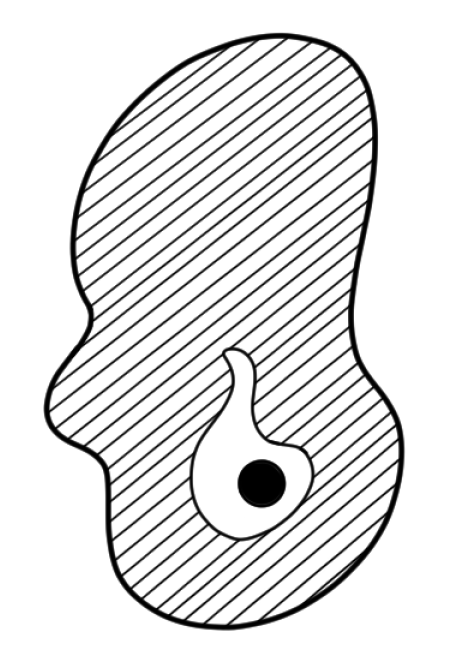
\includegraphics[width=0.3\linewidth]{./addons/starComplement.png}
			\end{tikzfigure}
			\vspace{1em}
			An operator $^\bullet$ is called \textit{co-$\star$-complement} if instead of $a^*\cap a=\emptyset$ we requires $a^\bullet\cup a=X$. Notice that if $^\bullet$ is a co-$\star$-complement then we can construct $\star$-complement operator by surrounding it by the complement: the map $a\mapsto a^{\complement\bullet\complement}$ is $\star$-complement and vice versa. This gives us a canonical correspondence between the co-$\star$-complement and the $\star$-complement.
			
			One can show by induction that if $^*$ is a $\star$-complement and $a\subseteq X$ is finite or cofinite, then $a^*=a^\complement$, so if there exists a $\star$-complement operator on $X$ then $X$ must be infinite, furthermore $X$ cannot be amorphous.
			
			On the other hand, if $X$ is Dedekind infinite then there exists a $\star$-complement operator for $X$. We may assume $\mathbb Z\subseteq X$, now if $a\subseteq X$ is of the form $\{q\in \mathbb Z\mid q>z\}$ for some $z\in \mathbb Z$, then let $a^*=\{q\in\mathbb Z\mid q<z\}$, for $a=\{q\in\mathbb Z\mid q<z\}$ let $a^*=\{q\in \mathbb Z\mid q>z\}$, otherwise let $a^*=a^\complement$.
			
			So in $\sf ZFC$ a set has a $\star$-complement operator if and only if it is infinite.
			
			An operator $^*$ is called \textit{strongly $\star$-complement} if it as far from the complement operator as possible: it is a $\star$-complement operator that agrees with the complement operator exactly on the finite and cofinite subsets.
			
			In $\sf ZFC$ every infinite set has a strongly $\star$-complement operator.
		}
		
		\column{0.32}
		\block{{\fontsize{60}{50}\selectfont$\star$-}Finite}{
			It turns out that a cardinality $\frak n$ has $\star$-complement operator if and only if it is infinite in the sense of $(4)$.
			
			\begin{tikzfigure}[$\cdots\rightarrow a^{\complement *}\rightarrow a\rightarrow a^{*\complement}\rightarrow\cdots$]
				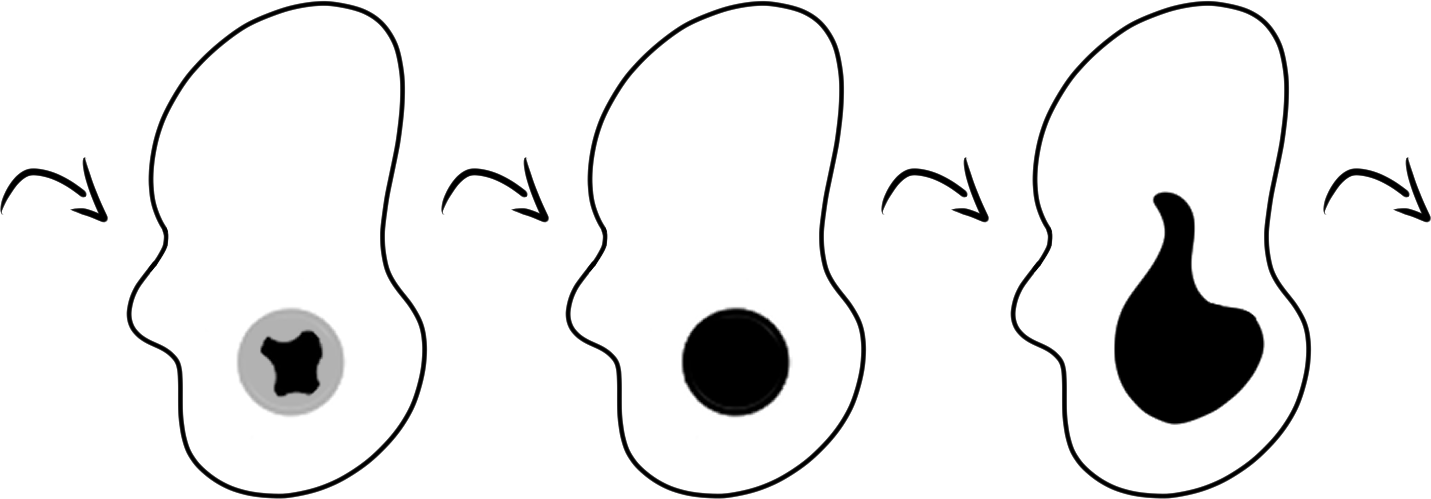
\includegraphics[width=0.4\linewidth]{./addons/Zembedding0.png}
			\end{tikzfigure}
			To see that we shall use the theorem of Kuratowski (see \cite{Tarski:0}), a cardinality is infinite in the sense of $(4)$ if and only if it surjects onto $\omega$. That in turn is equivalent to having $\mathcal U\subseteq \mathcal P(X)$ such that $(\mathcal U,\subset)\cong(\mathbb Z,<)$. To construct a $\star$-complement operator from being finite in the sense of $(4)$ we can replicate our construction from the previous part. 
			
			For the other direction let $^*$ be $\star$-complement and let $a$ be such that $a^*\ne a^\complement$, then we can repeat $^{*\complement}$ and $^{\complement *}$ to get a copy of $(\mathbb Z,<)$ (see figure $2$)
		}
		
		\block{Remarks}{
			\begin{enumerate}
				\addtolength{\itemindent}{0cm}
				\item A similar characteristic can be found for strongly $\star$-complement operator by finding partition of the infinite coinfinite subsets of $X$ into copies of $\mathbb Z$.
				\item It is not obvious if $\sf ZF$ proves that there exist sets with strongly $\star$-complement operators at all.
				\item Similarly to how we turn co-$\star$-complement operators into $\star$-complement operators, one can take a $\star$-complement operator and a co-$\star$-complement operator and produce a new $\star$-complement operator by $a\mapsto a^{\complement \bullet*}$.
			\end{enumerate}
		}
		
		%\block{Acknowledgements}{
		%	Lorem ipsum dolor sit amet, probo dolorem cu vis. Cu mei audire fabulas scriptorem, cu has clita fabulas. Sea id veritus maiorum indoctum, mea cu assum cetero. Ei posse movet maluisset vim.
		%}
		
		\block{References}{
			\vspace{-1em}
			\begin{footnotesize}
				\printbibliography[heading=none]
			\end{footnotesize}
		}
	\end{columns}
\end{document}